% !TeX document-id = {3323fc22-2641-4bde-b857-9c71dae59723}
% !TeX program = xelatex ?me -synctex=0 -interaction=nonstopmode -aux-directory=../tex_aux -output-directory=./release
% !TeX program = xelatex

\documentclass[12pt]{article}

\usepackage{lineno,changepage,lipsum}
\usepackage[colorlinks=true,urlcolor=blue]{hyperref}
\usepackage{fontspec}
\usepackage{xeCJK}
\usepackage{tabularx}
\setCJKfamilyfont{chanto}{AozoraMinchoRegular.ttf}
\setCJKfamilyfont{tegaki}{Mushin.otf}
\usepackage[CJK,overlap]{ruby}
\usepackage{hhline}
\usepackage{multirow,array,amssymb}
\usepackage[croatian]{babel}
\usepackage{soul}
\usepackage[usenames, dvipsnames]{color}
\usepackage{wrapfig,booktabs}
\renewcommand{\rubysep}{0.1ex}
\renewcommand{\rubysize}{0.75}
\usepackage[margin=50pt]{geometry}
\modulolinenumbers[2]

\usepackage{pifont}
\newcommand{\cmark}{\ding{51}}%
\newcommand{\xmark}{\ding{55}}%

\definecolor{faded}{RGB}{100, 100, 100}

\renewcommand{\arraystretch}{1.2}

%\ruby{}{}
%$($\href{URL}{text}$)$

\newcommand{\furigana}[2]{\ruby{#1}{#2}}
\newcommand{\tegaki}[1]{
	\CJKfamily{tegaki}\CJKnospace
	#1
	\CJKfamily{chanto}\CJKnospace
}

\newcommand{\dai}[1]{
	\vspace{20pt}
	\large
	\noindent\textbf{#1}
	\normalsize
	\vspace{20pt}
}

\newcommand{\fukudai}[1]{
	\vspace{10pt}
	\noindent\textbf{#1}
	\vspace{10pt}
}

\newenvironment{bunshou}{
	\vspace{10pt}
	\begin{adjustwidth}{1cm}{3cm}
	\begin{linenumbers}
}{
	\end{linenumbers}
	\end{adjustwidth}
}

\newenvironment{reibun}{
	\vspace{10pt}
	\begin{tabular}{l l}
}{
	\end{tabular}
	\vspace{10pt}
}
\newcommand{\rei}[2]{
	#1&\textit{#2}\\
}
\newcommand{\reinagai}[2]{
	\multicolumn{2}{l}{#1}\\
	\multicolumn{2}{l}{\hspace{10pt}\textit{#2}}\\
}

\newenvironment{mondai}[1]{
	\vspace{10pt}
	#1
	
	\begin{enumerate}
		\itemsep-5pt
	}{
	\end{enumerate}
	\vspace{10pt}
}

\newenvironment{hyou}{
	\begin{itemize}
		\itemsep-5pt
	}{
	\end{itemize}
	\vspace{10pt}
}

\date{\today}

\CJKfamily{chanto}\CJKnospace
\author{autor}
\begin{document}
	\dai{こどもの\furigana{日}{ひ}}

	\fukudai{lagani dio}
	\begin{bunshou}
		\hspace{15pt}日本では、5月5日は「こどもの日」と\furigana{言}{い}う\hspace{5pt}\furigana{祝日}{しゅくじつ}です。\furigana{昔}{むかし}は\hspace{10pt}\furigana{男}{おとこ}の\furigana{子}{こ}の\furigana{健}{すこ}やかな\furigana{成長}{せいちょう}を\hspace{10pt}\furigana{祈}{いの}る日でした。\hspace{5pt}1948\furigana{年}{ねん}に\furigana{名前}{なまえ}が「\furigana{端午の節句}{たんごのせっく}」から今のこどもの日に\furigana{変}{か}わって、男の子の日だけではなくなりました。

		それでも、\furigana{昔}{むかし}\hspace{10pt}\furigana{使}{つか}っていた\furigana{飾}{かざ}りは今も\furigana{飾}{かざ}ります。\hspace{5pt}\furigana{侍}{さむらい}の\hspace{10pt}\furigana{鎧}{よろい}や\hspace{10pt}\furigana{兜}{かぶと}、そして\furigana{鯉}{こい}のぼり。
	\end{bunshou}

	\fukudai{teži dio}
	\begin{bunshou}
		さて、どうして鯉のぼりを飾るようになりましたか。

		\furigana{江戸時代}{えどじだい}の\furigana{武家}{ぶけ}に男の子が生まれた時、のぼりを飾る\furigana{習慣}{しゅうかん}がありましたが、それは鯉のぼりではありませんでした (Slika 2)。のちに川をさかのぼる鯉は\furigana{出世}{しゅっせ}の\hspace{10pt}\furigana{象徴}{しょうちょう}となって、「のぼる鯉」が「鯉のぼり」になりました。
	\end{bunshou}

	\begin{figure}[h]
		\centering
		\begin{minipage}{.45\textwidth}
			\centering
			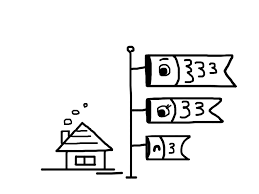
\includegraphics[width=\textwidth]{00x_citanje_tango_res/koinobori}
			\caption{鯉のぼり}
		\end{minipage}
		\begin{minipage}{.45\textwidth}
			\centering
			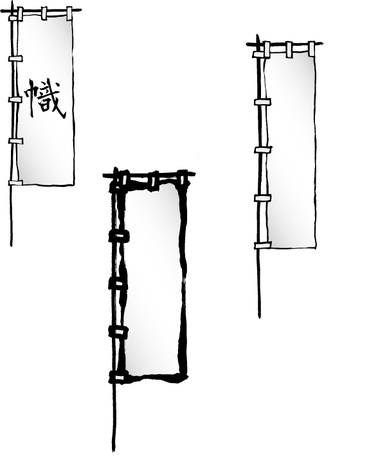
\includegraphics[width=.6\textwidth]{00x_citanje_tango_res/nobori}
			\caption{のぼり}
		\end{minipage}
	\end{figure}

	\newpage
	\fukudai{Pitanja}

	\begin{mondai}{Lakši dio:}
		\item この\furigana{文章}{ぶんしょう}は\hspace{10pt}\furigana{難}{むず}しかったですか。
		\item 「5月5日」はどう\furigana{読}{よ}みますか。
		\item 「1948年」は?
		\item こどもの日の\furigana{昔}{むかし}の\furigana{名前}{なまえ}は\furigana{何}{なん}ですか。
		\item こどもの日にはどんな\furigana{飾}{かざ}りを\furigana{飾}{かざ}りますか。
		\item ゴールデンウィーク、\furigana{知}{し}っていますか。
	\end{mondai}

	\begin{mondai}{Teži dio:}
		\item この文章は難しかったですか。
		\item 昔の「のぼり」は何ですか。
	\end{mondai}
	\fukudai{Nepoznate riječi}

	\begin{tabular}{l l l l}
		\furigana{祝日}{しゅくじつ}&\textit{praznik}&\furigana{昔}{むかし}&\textit{davno} (kao pril. ozn. vremena)\\
		\furigana{健}{すこ}やか&\textit{zdravo}, \textit{čilo}&\furigana{成長}{せいうちょう}&\textit{rast}\\
		\furigana{祈}{いの}る&\textit{moliti se} (komeに za štoを)&\furigana{変}{か}わる&\textit{promijeniti se\footnotemark[1]}\\
		\furigana{使}{つか}う&\textit{koristiti}&\furigana{飾}{かざ}り&\textit{ukras}\\
		\furigana{飾}{かざ}る&\textit{staviti za ukras}&\furigana{鎧}{よろい}&\textit{oklop}\\
		\furigana{兜}{かぶと}&\textit{samurajska kaciga}&\furigana{鯉}{こい}&\textit{šaran}\\
		のぼる&\textit{penjati se}&鯉のぼり&\textit{posebni ukrasi} (vidi sliku 1)\\
		のぼり&\textit{zastava}&\furigana{江戸時代}{えどじだい}&period 1603\textasciitilde1868\\
		\furigana{武家}{ぶけ}&\textit{ratnička (samurajska) obitelj}&\furigana{習慣}{しゅうかん}&\textit{običaj}\\
		さかのぼる&\textit{plivati uzvodno}&出世&\textit{uspon u društvu}\\
		\furigana{象徴}{しょうちょう}&\textit{simbol}&&\\
	\end{tabular}
	\footnotetext[1]{Pijelazna verzija je \textit{što}を 変える.}
\end{document}
